\documentclass[12pt, a4paper]{article}

% ── Packages ──────────────────────────────────────────────────────
\usepackage{fontspec}
\setmainfont{Sylfaen}
\usepackage{amsmath, amssymb, amsthm}
\renewcommand\proofname{Ապացույց}
\usepackage{mathtools}
\usepackage{enumitem}
\usepackage{tikz}
\usetikzlibrary{calc, positioning, arrows.meta, fit, patterns, decorations.pathreplacing}
\usepackage{geometry}
\geometry{margin=2.4cm}
\usepackage{xcolor}
\usepackage{tcolorbox}
\tcbuselibrary{theorems, skins, breakable}
\usepackage{booktabs}
\usepackage{hyperref}
\hypersetup{colorlinks=true, linkcolor=blue!60!black, urlcolor=blue!60!black}

\setlength{\parindent}{0pt}
\setlength{\parskip}{6pt}

% ── Colours ───────────────────────────────────────────────────────
\definecolor{setA}{RGB}{66, 133, 244}   % blue
\definecolor{setB}{RGB}{234, 67, 53}    % red
\definecolor{setC}{RGB}{251, 188, 4}    % yellow
\definecolor{theoryBg}{RGB}{232, 245, 253}
\definecolor{theoryFrame}{RGB}{66, 133, 244}
\definecolor{stmtBg}{RGB}{255, 243, 224}
\definecolor{stmtFrame}{RGB}{230, 126, 34}
\definecolor{ansBg}{RGB}{232, 250, 232}
\definecolor{ansFrame}{RGB}{39, 174, 96}

% ── Environments ──────────────────────────────────────────────────
\newtcolorbox{theorybox}[1][]{%
  colback=theoryBg, colframe=theoryFrame,
  fonttitle=\bfseries, title={\small Տեսության ամփոփում. #1},
  breakable, enhanced, arc=2mm,
  left=5pt, right=5pt, top=5pt, bottom=5pt
}

\newtcolorbox{problembox}{%
  colback=stmtBg, colframe=stmtFrame,
  fonttitle=\bfseries, title={\small Խնդրի դրվածք},
  breakable, enhanced, arc=2mm,
  left=5pt, right=5pt, top=5pt, bottom=5pt
}

\newtcolorbox{answerbox}{%
  colback=ansBg, colframe=ansFrame,
  arc=2mm, left=5pt, right=5pt, top=3pt, bottom=3pt
}

\newcommand{\Z}{\mathbb{Z}}
\newcommand{\R}{\mathbb{R}}
\newcommand{\N}{\mathbb{N}}
\newcommand{\Q}{\mathbb{Q}}
\newcommand{\powset}[1]{2^{#1}}
\newcommand{\comp}[1]{\overline{#1}}
\newcommand{\symdiff}{\mathbin{\triangle}}

% ── Title ─────────────────────────────────────────────────────────
\title{\textbf{Գործնական 4 — Ֆունկցիաներ (արտապատկերումներ)}\\[4pt]
       \large Ընտրված խնդիրների լուծումներ\\[2pt]
       \normalsize Խնդիրներ 2, 4, 5, 6, 10, 12, 19, 22, 24, 25}
\author{Դիսկրետ մաթեմատիկա — ԵՊՀ}
\date{}

\begin{document}
\maketitle
\tableofcontents
\newpage

% ══════════════════════════════════════════════════════════════════
\section{Խնդիր 2 — Իրական ֆունկցիաների որոշման և արժեքների տիրույթներ}
% ══════════════════════════════════════════════════════════════════

\begin{theorybox}[Որոշման և Արժեքների տիրույթներ]
$f(x) = \ldots$ բանաձևով տրված $f : \R \to \R$ ֆունկցիայի համար․
\begin{itemize}[nosep]
  \item \textbf{Որոշման տիրույթը}՝ $\operatorname{Dom}(f)$-ը, բոլոր այն $x \in \R$ թվերի բազմությունն է,
        որոնց համար բանաձևը իմաստ ունի (բաժանում զրոյի վրա չկա, բացասական թվից քառակուսի արմատ չկա, և այլն)։
  \item \textbf{Արժեքների տիրույթը}՝ $\operatorname{Ran}(f) = \{f(x) \mid x \in \operatorname{Dom}(f)\}$-ը, 
        այն բոլոր արժեքների բազմությունն է, որոնք ֆունկցիան փաստացի ընդունում է։
\end{itemize}

\medskip
\textbf{Հաճախ հանդիպող սահմանափակումներ.}
\begin{center}
\renewcommand{\arraystretch}{1.3}
\begin{tabular}{lll}
\toprule
\textbf{Արտահայտություն} & \textbf{Սահմանափակում} & \textbf{Պատճառ} \\
\midrule
$\sqrt{g(x)}$ & $g(x) \ge 0$ & բացասական թվի արմատը անորոշ է $\R$-ում \\
$1/g(x)$ & $g(x) \neq 0$ & բաժանում զրոյի վրա անթույլատրելի է \\
$1/\sqrt{g(x)}$ & $g(x) > 0$ & երկու սահմանափակումները միասին \\
\bottomrule
\end{tabular}
\end{center}
\end{theorybox}

\begin{problembox}
Դիցուք $f : \R \to \R$։ Գտեք հետևյալ ֆունկցիաների որոշման և արժեքների տիրույթները․
\begin{enumerate}[label=(\alph*), nosep]
  \item $f(x) = x^2 + 3$
  \item $f(x) = \sqrt{x+2}$
  \item $f(x) = \dfrac{1}{\sqrt{x-2}}$
  \item $f(x) = |x|$
  \item $f(x) = \dfrac{1}{x^2+2}$
  \item $f(x) = \dfrac{1}{x^2-2}$
\end{enumerate}
\end{problembox}

\subsection*{Լուծում}

\textbf{Երկու քայլ յուրաքանչյուր արտապատկերման համար.}
\begin{enumerate}[nosep]
  \item \textbf{Որոշման տիրույթի ստուգում.} որոշեք, թե որտեղ է բանաձևը որոշված։
  \item \textbf{Արժեքների տիրույթի ստուգում.} որոշեք, թե որ ելքային արժեքներն են ստացվում։
\end{enumerate}

\medskip

\textbf{(a)\; $f(x) = x^2 + 3$.}

$x$-ի վրա սահմանափակումներ չկան․ ցանկացած իրական թիվ կարելի է բարձրացնել քառակուսի։
\[
  \operatorname{Dom}(f) = \R.
\]
Քանի որ $x^2 \ge 0$ բոլոր $x \in \R$-ի համար, ունենք $f(x) = x^2 + 3 \ge 3$։
Նվազագույն արժեքը՝ $3$-ը, ստացվում է $x = 0$ կետում։
Երբ $x \to \pm\infty$, $f(x) \to +\infty$, և անընդհատության շնորհիվ բոլոր $\ge 3$ արժեքները ընդունվում են։
\[
  \operatorname{Ran}(f) = [3, +\infty).
\]

\begin{answerbox}
$\operatorname{Dom}(f) = \R, \quad \operatorname{Ran}(f) = [3, +\infty).$
\end{answerbox}

\bigskip
\textbf{(b)\; $f(x) = \sqrt{x+2}$.}

Մեզ պետք է $x + 2 \ge 0$, այսինքն՝ $x \ge -2$։
\[
  \operatorname{Dom}(f) = [-2, +\infty).
\]
$x = -2$ դեպքում՝ $f(-2) = 0$։ Երբ $x \to +\infty$, $f(x) \to +\infty$։
Քանի որ $\sqrt{\cdot}$-ը անընդհատ է և ոչ բացասական․
\[
  \operatorname{Ran}(f) = [0, +\infty).
\]

\begin{answerbox}
$\operatorname{Dom}(f) = [-2, +\infty), \quad \operatorname{Ran}(f) = [0, +\infty).$
\end{answerbox}

\bigskip
\textbf{(c)\; $f(x) = \dfrac{1}{\sqrt{x-2}}$.}

Մեզ պետք է $x - 2 > 0$ (խիստ անհավասարություն․ արմատի տակը դրական է, քանի որ այն հայտարարում է), այսինքն՝ $x > 2$։
\[
  \operatorname{Dom}(f) = (2, +\infty).
\]
Երբ $x \to 2^+$՝ $\sqrt{x-2} \to 0^+$, ուստի $f(x) \to +\infty$։
Երբ $x \to +\infty$՝ $\sqrt{x-2} \to +\infty$, ուստի $f(x) \to 0^+$։
Քանի որ $f$-ը անընդհատ է և խիստ նվազող $(2, +\infty)$-ում, այն ընդունում է բոլոր դրական արժեքները․
\[
  \operatorname{Ran}(f) = (0, +\infty).
\]

\begin{answerbox}
$\operatorname{Dom}(f) = (2, +\infty), \quad \operatorname{Ran}(f) = (0, +\infty).$
\end{answerbox}

\bigskip
\textbf{(d)\; $f(x) = |x|$.}

Բացարձակ արժեքը որոշված է բոլոր իրական թվերի համար։
\[
  \operatorname{Dom}(f) = \R.
\]
Քանի որ $|x| \ge 0$ բոլոր $x$-երի համար, և $|0| = 0$, ու $|x| \to +\infty$ երբ $x \to \pm\infty$․
\[
  \operatorname{Ran}(f) = [0, +\infty).
\]

\begin{answerbox}
$\operatorname{Dom}(f) = \R, \quad \operatorname{Ran}(f) = [0, +\infty).$
\end{answerbox}

\bigskip
\textbf{(e)\; $f(x) = \dfrac{1}{x^2+2}$.}

Քանի որ $x^2 + 2 \ge 2 > 0$ բոլոր $x \in \R$-ի համար, զրոյի բաժանում չկա։
\[
  \operatorname{Dom}(f) = \R.
\]
Քանի որ $x^2 + 2 \ge 2$, ունենք $f(x) = \frac{1}{x^2+2} \le \frac{1}{2}$։
Առավելագույն արժեքը՝ $\frac{1}{2}$-ը, ստացվում է $x = 0$ կետում։
Երբ $x \to \pm\infty$, $f(x) \to 0^+$, բայց $f(x) > 0$ բոլոր $x$-երի համար։
Ըստ անընդհատության, $(0, \frac{1}{2}]$ միջակայքի բոլոր արժեքները ընդունվում են։
\[
  \operatorname{Ran}(f) = \left(0,\; \tfrac{1}{2}\right].
\]

\begin{answerbox}
$\operatorname{Dom}(f) = \R, \quad \operatorname{Ran}(f) = \bigl(0,\, \frac{1}{2}\bigr].$
\end{answerbox}

\bigskip
\textbf{(f)\; $f(x) = \dfrac{1}{x^2-2}$.}

Մեզ պետք է $x^2 - 2 \neq 0$, այսինքն՝ $x \neq \pm\sqrt{2}$։
\[
  \operatorname{Dom}(f) = \R \setminus \{-\sqrt{2},\; \sqrt{2}\}.
\]
Արժեքների տիրույթը գտնելու համար նշանակենք $y = \frac{1}{x^2 - 2}$ և լուծենք $x^2$-ու համար․
\[
  y(x^2 - 2) = 1 \implies x^2 = \frac{1}{y} + 2 = \frac{1 + 2y}{y}.
\]
Մեզ պետք է $y \neq 0$ և $x^2 = \frac{1+2y}{y} \ge 0$։

\textbf{Նշանների վերլուծություն.}\; $x^2 = \frac{1+2y}{y} \ge 0$ լուծելու համար համարիչն ու հայտարարը պետք է ունենան նույն նշանը։ $y > 0$-ի դեպքում՝ $1+2y > 0$ միշտ, ուստի բոլոր $y > 0$-ները բավարարում են։ $y < 0$-ի դեպքում՝ պետք է $1+2y < 0$, այսինքն՝ $y < -\tfrac{1}{2}$։ Հետևաբար $y \in (-\infty, -\tfrac{1}{2}) \cup (0, +\infty)$, գումարած՝ պետք է ստուգել եզրային կետերը։

$x = 0$ դեպքում՝ $f(0) = \frac{1}{-2} = -\frac{1}{2}$, ուստի $y = -\frac{1}{2}$ արժեքը ընդունվում է։
\[
  \operatorname{Ran}(f) = \left(-\infty,\; -\tfrac{1}{2}\right] \cup (0, +\infty).
\]

\begin{answerbox}
$\operatorname{Dom}(f) = \R \setminus \{-\sqrt{2},\, \sqrt{2}\}, \quad
 \operatorname{Ran}(f) = \bigl(-\infty,\, -\tfrac{1}{2}\bigr] \cup (0, +\infty).$
\end{answerbox}

% ══════════════════════════════════════════════════════════════════
\newpage
\section{Խնդիր 4 — Ֆունկցիաների կոմպոզիցիա}
% ══════════════════════════════════════════════════════════════════

\begin{theorybox}[Ֆունկցիաների կոմպոզիցիա]
Տրված $f, g : \R \to \R$ ֆունկցիաների համար $f \circ g$ \textbf{կոմպոզիցիան} սահմանվում է․
\[
  (f \circ g)(x) = f\bigl(g(x)\bigr).
\]
\textbf{Կարդացեք աջից ձախ.} նախ կիրառեք $g$-ն, հետո ստացված արդյունքի վրա կիրառեք $f$-ը։

\begin{center}
\begin{tikzpicture}[>=Stealth, font=\small, node distance=2.5cm]
  \node[draw, rounded corners, fill=setA!10, minimum width=1.4cm, minimum height=0.9cm] (X) {$x$};
  \node[draw, rounded corners, fill=setC!15, minimum width=1.4cm, minimum height=0.9cm, right=of X] (GX) {$g(x)$};
  \node[draw, rounded corners, fill=setB!10, minimum width=1.4cm, minimum height=0.9cm, right=of GX] (FGX) {$f(g(x))$};
  \draw[->, thick, setA!70!black] (X) -- (GX)
    node[midway, above, font=\footnotesize]{կիրառել $g$};
  \draw[->, thick, setB!70!black] (GX) -- (FGX)
    node[midway, above, font=\footnotesize]{կիրառել $f$};
  \draw[->, thick, gray, dashed, bend left=30] (X) to
    node[midway, below=6pt, font=\footnotesize]{$f \circ g$} (FGX);
\end{tikzpicture}
\end{center}

\textbf{Զգուշացում.} Ընդհանուր դեպքում $f \circ g \neq g \circ f$ — կոմպոզիցիան կոմուտատիվ (տեղափոխական) չէ։
\end{theorybox}

\begin{problembox}
Դիցուք $f, g : \R \to \R$։ Գտեք $f \circ g$-ն և $g \circ f$-ը, եթե․
\begin{enumerate}[label=(\alph*), nosep]
  \item $f(x) = x^2 + 1$, \quad $g(x) = x + 3$
  \item $f(x) = \sqrt{x^2 + 2}$, \quad $g(x) = x^2 + 3$
  \item $f(x) = \dfrac{1}{x}$, \quad $g(x) = 2x + 3$
\end{enumerate}
\end{problembox}

\subsection*{Լուծում}

\textbf{(a)\; $f(x) = x^2 + 1$, \;$g(x) = x + 3$.}

\[
  (f \circ g)(x) = f(g(x)) = f(x+3) = (x+3)^2 + 1 = x^2 + 6x + 9 + 1 = x^2 + 6x + 10.
\]
\[
  (g \circ f)(x) = g(f(x)) = g(x^2+1) = (x^2+1) + 3 = x^2 + 4.
\]

\begin{answerbox}
$(f \circ g)(x) = x^2 + 6x + 10, \qquad (g \circ f)(x) = x^2 + 4.$
\end{answerbox}

\bigskip
\textbf{(b)\; $f(x) = \sqrt{x^2 + 2}$, \;$g(x) = x^2 + 3$.}

\[
  (f \circ g)(x) = f(g(x)) = f(x^2 + 3) = \sqrt{(x^2+3)^2 + 2} = \sqrt{x^4 + 6x^2 + 9 + 2} = \sqrt{x^4 + 6x^2 + 11}.
\]
\[
  (g \circ f)(x) = g(f(x)) = g\!\left(\sqrt{x^2+2}\right) = \left(\sqrt{x^2+2}\right)^2 + 3 = x^2 + 2 + 3 = x^2 + 5.
\]

\begin{answerbox}
$(f \circ g)(x) = \sqrt{x^4 + 6x^2 + 11}, \qquad (g \circ f)(x) = x^2 + 5.$
\end{answerbox}

\bigskip
\textbf{(c)\; $f(x) = \dfrac{1}{x}$, \;$g(x) = 2x + 3$.}

\[
  (f \circ g)(x) = f(g(x)) = f(2x+3) = \frac{1}{2x+3}, \qquad x \neq -\tfrac{3}{2}.
\]
\[
  (g \circ f)(x) = g(f(x)) = g\!\left(\frac{1}{x}\right) = \frac{2}{x} + 3 = \frac{2 + 3x}{x}, \qquad x \neq 0.
\]

\textbf{Որոշման տիրույթի ստուգում.}\; Բանաձևը հաշվելուց հետո ստուգեք, թե որտեղ է այն որոշված․ $(g \circ f)(x)$-ի համար պահանջվում է $x \in \operatorname{Dom}(f)$ և $f(x) \in \operatorname{dom}(g)$։

\begin{answerbox}
$(f \circ g)(x) = \dfrac{1}{2x+3}\;(x \neq -\frac{3}{2}), \qquad
 (g \circ f)(x) = \dfrac{2+3x}{x}\;(x \neq 0).$
\end{answerbox}

% ══════════════════════════════════════════════════════════════════
\newpage
\section{Խնդիր 5 — Հակադարձ ֆունկցիաներ}
% ══════════════════════════════════════════════════════════════════

\begin{theorybox}[Հակադարձ ֆունկցիա]
Եթե $f : A \to B$-ն բիյեկցիա է, ապա $f$-ն ունի \textbf{հակադարձ ֆունկցիա}՝ $f^{-1} : B \to A$, որը բավարարում է․
\[
  f^{-1}(y) = x \iff f(x) = y.
\]
\textbf{$f^{-1}$-ը գտնելու ալգորիթմ.}
\begin{enumerate}[nosep]
  \item Գրեք $y = f(x)$։
  \item Լուծեք $x$-ը $y$-ի միջոցով։
  \item Փոխեք անունները․ ստացված $x$-ի արտահայտությունը $y$-ից հենց $f^{-1}(y)$-ն է։
\end{enumerate}

\textbf{Ստուգում.} $f^{-1}(f(x)) = x$ և $f(f^{-1}(y)) = y$։
\end{theorybox}

\begin{problembox}
Գտեք հակադարձ հարաբերությունը․
\begin{enumerate}[label=(\alph*), nosep]
  \item $f(x) = \dfrac{x+4}{2}$
  \item $f(x) = x^3$
  \item $f(x) = \dfrac{x-2}{x+3}$
\end{enumerate}
\end{problembox}

\subsection*{Լուծում}

\textbf{(a)\; $f(x) = \dfrac{x+4}{2}$.}

Նշանակեք $y = \frac{x+4}{2}$։ Լուծեք $x$-ի համար․
\[
  2y = x + 4 \implies x = 2y - 4.
\]
\[
  \boxed{f^{-1}(y) = 2y - 4.}
\]

\emph{Ստուգում՝}\; $f(f^{-1}(y)) = f(2y-4) = \frac{(2y-4)+4}{2} = \frac{2y}{2} = y.\;\checkmark$

$f^{-1}(f(x)) = f^{-1}\!\left(\frac{x+4}{2}\right) = 2 \cdot \frac{x+4}{2} - 4 = x + 4 - 4 = x.\;\checkmark$

\begin{answerbox}
$f^{-1}(x) = 2x - 4.$
\end{answerbox}

\bigskip
\textbf{(b)\; $f(x) = x^3$.}

Նշանակեք $y = x^3$։ Լուծեք $x$-ի համար․
\[
  x = \sqrt[3]{y} = y^{1/3}.
\]
\[
  \boxed{f^{-1}(y) = \sqrt[3]{y}.}
\]

\emph{Ստուգում՝}\; $f(f^{-1}(y)) = (\sqrt[3]{y})^3 = y.\;\checkmark$ \quad
$f^{-1}(f(x)) = \sqrt[3]{x^3} = x.\;\checkmark$

\begin{answerbox}
$f^{-1}(x) = \sqrt[3]{x}.$
\end{answerbox}

\bigskip
\textbf{(c)\; $f(x) = \dfrac{x-2}{x+3}$, \quad $x \neq -3$.}

Նշանակեք $y = \frac{x-2}{x+3}$։ Լուծեք $x$-ի համար․
\begin{align*}
  y(x+3) &= x - 2 \\
  yx + 3y &= x - 2 \\
  yx - x &= -2 - 3y \\
  x(y - 1) &= -(2 + 3y) \\
  x &= \frac{-(2+3y)}{y-1} = \frac{2+3y}{1-y}, \qquad y \neq 1.
\end{align*}
Նկատենք, որ $f(x) = 1$ հավասարումը լուծում չունի (դա կպահանջեր $x - 2 = x + 3$, այսինքն՝ $-2 = 3$), ինչը հաստատում է, որ $1 \notin \operatorname{Ran}(f)$։
\[
  \boxed{f^{-1}(y) = \frac{2 + 3y}{1 - y}, \qquad y \neq 1.}
\]

\emph{Ստուգում՝}\;
$f(f^{-1}(y)) = f\!\left(\frac{2+3y}{1-y}\right)
= \frac{\frac{2+3y}{1-y} - 2}{\frac{2+3y}{1-y} + 3}
= \frac{2+3y - 2(1-y)}{2+3y + 3(1-y)}
= \frac{2+3y-2+2y}{2+3y+3-3y}
= \frac{5y}{5} = y.\;\checkmark$

\begin{answerbox}
$f^{-1}(x) = \dfrac{2+3x}{1-x}, \quad x \neq 1.$
\end{answerbox}

\bigskip
\textbf{Նշում.}\; Այստեղ հակադարձ հարաբերությունը ստացվում է ֆունկցիա, քանի որ յուրաքանչյուր արտապատկերում բիյեկտիվ է իր արժեքների տիրույթի վրա։ Ընդհանուր դեպքում հակադարձ \emph{հարաբերությունը} միշտ գոյություն ունի, բայց այն \emph{ֆունկցիա} է միայն այն դեպքում, երբ սկզբնական արտապատկերումը ինյեկտիվ է։

% ══════════════════════════════════════════════════════════════════
\newpage
\section{Խնդիր 6 — Ինյեկտիվություն, Սյուրյեկտիվություն, Բիյեկտիվություն}
% ══════════════════════════════════════════════════════════════════

\begin{theorybox}[Ինյեկտիվ, Սյուրյեկտիվ, Բիյեկտիվ]
Դիցուք $f : A \to B$։
\begin{itemize}[nosep]
  \item \textbf{Ինյեկտիվ} (միարժեք). $f(x_1) = f(x_2) \implies x_1 = x_2$։
        Համարժեքորեն, $x_1 \neq x_2 \implies f(x_1) \neq f(x_2)$։
        \emph{Հորիզոնական գծի թեստ.} յուրաքանչյուր հորիզոնական գիծ հատում է գրաֆիկը առավելագույնը մեկ անգամ։
  \item \textbf{Սյուրյեկտիվ} (վերարժեք, «onto»). $\forall\, y \in B,\; \exists\, x \in A : f(x) = y$։
        Համարժեքորեն, $\operatorname{Ran}(f) = B$։
  \item \textbf{Բիյեկտիվ} (փոխմիարժեք). թե՛ ինյեկտիվ, թե՛ սյուրյեկտիվ։
\end{itemize}

\begin{center}
\begin{tikzpicture}[>=Stealth, font=\small]
  % Injective
  \begin{scope}[xshift=0cm]
    \node[font=\footnotesize\bfseries] at (1.2, 2.5) {Ինյեկտիվ};
    \draw[thick, rounded corners] (0, -0.3) rectangle (0.8, 2.1);
    \draw[thick, rounded corners] (1.6, -0.3) rectangle (2.4, 2.1);
    \node[font=\scriptsize] at (0.4, -0.6) {$A$};
    \node[font=\scriptsize] at (2.0, -0.6) {$B$};
    \foreach \y/\lbl in {0.3/a, 0.9/b, 1.5/c}
      \node[fill=setA!30, circle, inner sep=1.5pt, font=\tiny] (L\lbl) at (0.4, \y) {\lbl};
    \foreach \y/\lbl in {0.0/1, 0.6/2, 1.2/3, 1.8/4}
      \node[fill=setB!20, circle, inner sep=1.5pt, font=\tiny] (R\lbl) at (2.0, \y) {\lbl};
    \draw[->, thick, gray] (La) -- (R1);
    \draw[->, thick, gray] (Lb) -- (R3);
    \draw[->, thick, gray] (Lc) -- (R4);
  \end{scope}
  % Surjective
  \begin{scope}[xshift=4cm]
    \node[font=\footnotesize\bfseries] at (1.2, 2.5) {Սյուրյեկտիվ};
    \draw[thick, rounded corners] (0, -0.3) rectangle (0.8, 2.1);
    \draw[thick, rounded corners] (1.6, -0.3) rectangle (2.4, 2.1);
    \node[font=\scriptsize] at (0.4, -0.6) {$A$};
    \node[font=\scriptsize] at (2.0, -0.6) {$B$};
    \foreach \y/\lbl in {0.2/a, 0.7/b, 1.2/c, 1.7/d}
      \node[fill=setA!30, circle, inner sep=1.5pt, font=\tiny] (L\lbl) at (0.4, \y) {\lbl};
    \foreach \y/\lbl in {0.3/1, 0.9/2, 1.5/3}
      \node[fill=setB!20, circle, inner sep=1.5pt, font=\tiny] (R\lbl) at (2.0, \y) {\lbl};
    \draw[->, thick, gray] (La) -- (R1);
    \draw[->, thick, gray] (Lb) -- (R2);
    \draw[->, thick, gray] (Lc) -- (R3);
    \draw[->, thick, gray] (Ld) -- (R2);
  \end{scope}
  % Bijective
  \begin{scope}[xshift=8cm]
    \node[font=\footnotesize\bfseries] at (1.2, 2.5) {Բիյեկտիվ};
    \draw[thick, rounded corners] (0, -0.3) rectangle (0.8, 2.1);
    \draw[thick, rounded corners] (1.6, -0.3) rectangle (2.4, 2.1);
    \node[font=\scriptsize] at (0.4, -0.6) {$A$};
    \node[font=\scriptsize] at (2.0, -0.6) {$B$};
    \foreach \y/\lbl in {0.3/a, 0.9/b, 1.5/c}
      \node[fill=setA!30, circle, inner sep=1.5pt, font=\tiny] (L\lbl) at (0.4, \y) {\lbl};
    \foreach \y/\lbl in {0.3/1, 0.9/2, 1.5/3}
      \node[fill=setB!20, circle, inner sep=1.5pt, font=\tiny] (R\lbl) at (2.0, \y) {\lbl};
    \draw[->, thick, gray] (La) -- (R1);
    \draw[->, thick, gray] (Lb) -- (R2);
    \draw[->, thick, gray] (Lc) -- (R3);
  \end{scope}
\end{tikzpicture}
\end{center}
\end{theorybox}

\begin{problembox}
Որոշեք, թե հետևյալ $f : \R \to \R$ արտապատկերումներից որոնք են ինյեկտիվ, սյուրյեկտիվ կամ բիյեկտիվ.
\begin{enumerate}[label=(\alph*), nosep]
  \item $f(x) = |x|$
  \item $f(x) = x^2 + 4$
  \item $f(x) = x^3 + 6$
  \item $f(x) = x + |x|$
  \item $f(x) = x(x-2)(x+2)$
\end{enumerate}
\end{problembox}

\subsection*{Լուծում}

\textbf{Արագ թեստեր.}
\begin{itemize}[nosep]
  \item $|x|$: սիմետրիան ($f(x) = f(-x)$) անմիջապես ցույց է տալիս, որ ինյեկտիվ չէ։
  \item $x^2 + c$: պարաբոլը ունի մինիմում, ուստի սյուրյեկտիվ չէ $\mathbb{R}$-ի վրա։
  \item $x^3 + c$: խիստ մոնոտոն է, հետևաբար ինյեկտիվ է; սահմանային վարքը տալիս է սյուրյեկտիվություն։
  \item $x + |x|$: նախ վերածեք կտորային տեսքի, հետո ստուգեք յուրաքանչյուր կտորը։
  \item $x^3 - 4x$: փնտրեք կրկնվող արժեքներ (լոկալ էքստրեմումներ) և օգտագործեք սահմանային վարքը սյուրյեկտիվության համար։
\end{itemize}

\medskip

\textbf{(a)\; $f(x) = |x|$.}

\emph{Ինյեկտիվ չէ՝}\; $f(1) = |1| = 1 = |-1| = f(-1)$, բայց $1 \neq -1$։

\emph{Սյուրյեկտիվ չէ՝}\; $|x| \ge 0$ բոլոր $x$-երի համար, ուստի ոչ մի $x$ չի բավարարում $f(x) = -1$։
Արժեքների տիրույթը $[0, +\infty) \neq \R$ է։

\begin{answerbox}
$f(x) = |x|$: ոչ ինյեկտիվ է, ոչ էլ սյուրյեկտիվ (հետևաբար բիյեկտիվ չէ)։
\end{answerbox}

\bigskip
\textbf{(b)\; $f(x) = x^2 + 4$.}

\emph{Ինյեկտիվ չէ՝}\; $f(1) = 5 = f(-1)$, բայց $1 \neq -1$։

\emph{Սյուրյեկտիվ չէ՝}\; $x^2 + 4 \ge 4$ բոլոր $x$-երի համար, ուստի ոչ մի $x$ չի բավարարում $f(x) = 0$։
Արժեքների տիրույթը $[4, +\infty) \neq \R$ է։

\begin{answerbox}
$f(x) = x^2 + 4$: ոչ ինյեկտիվ է, ոչ էլ սյուրյեկտիվ (հետևաբար բիյեկտիվ չէ)։
\end{answerbox}

\bigskip
\textbf{(c)\; $f(x) = x^3 + 6$.}

\emph{Ինյեկտիվ է՝}\; Դիցուք $f(x_1) = f(x_2)$։ Այդ դեպքում $x_1^3 + 6 = x_2^3 + 6$,
ուստի $x_1^3 = x_2^3$։ Քանի որ խորանարդ ֆունկցիան խիստ աճող է $\R$-ում,
սրանից հետևում է $x_1 = x_2$։

\emph{Սյուրյեկտիվ է՝}\; Ցանկացած $y \in \R$-ի համար, մեզ պետք է $x^3 + 6 = y$, այսինքն՝
$x = \sqrt[3]{y - 6}$։ Քանի որ խորանարդ արմատը որոշված է բոլոր իրական թվերի համար, ապա
այդպիսի $x$ միշտ գոյություն ունի։

\begin{answerbox}
$f(x) = x^3 + 6$: \textbf{բիյեկտիվ} է (և՛ ինյեկտիվ, և՛ սյուրյեկտիվ)։
\end{answerbox}

\bigskip
\textbf{(d)\; $f(x) = x + |x|$.}

Նախ պարզեցնենք․
\[
  f(x) = x + |x| = \begin{cases} 2x & \text{եթե } x \ge 0, \\ 0 & \text{եթե } x < 0. \end{cases}
\]

\emph{Ինյեկտիվ չէ՝}\; $f(-1) = 0 = f(-2)$, բայց $-1 \neq -2$։
(Փաստացի, $f(x) = 0$ բոլոր $x < 0$-ների համար։)

\emph{Սյուրյեկտիվ չէ՝}\; $x \ge 0$-ի համար $f(x) = 2x \ge 0$։
$x < 0$-ի համար $f(x) = 0$։ Ուստի $f(x) \ge 0$ բոլոր $x$-երի համար,
և ոչ մի $x$ չի բավարարում $f(x) = -1$։ Արժեքների տիրույթը $[0, +\infty) \neq \R$ է։

\begin{answerbox}
$f(x) = x + |x|$: ոչ ինյեկտիվ է, ոչ էլ սյուրյեկտիվ (հետևաբար բիյեկտիվ չէ)։
\end{answerbox}

\bigskip
\textbf{(e)\; $f(x) = x(x-2)(x+2) = x^3 - 4x$.}

\emph{Ինյեկտիվ չէ՝}\; $f(0) = 0$ և $f(2) = 2 \cdot 0 \cdot 4 = 0$,
ուստի $f(0) = f(2) = 0$, բայց $0 \neq 2$։

\emph{Սյուրյեկտիվ է՝}\; $f(x) = x^3 - 4x$-ը խորանարդ բազմանդամ է դրական ավագ գործակցով։
Երբ $x \to -\infty$, $f(x) \to -\infty$, և երբ $x \to +\infty$, $f(x) \to +\infty$։
Միջանկյալ արժեքի թեորեմի համաձայն, յուրաքանչյուր $y \in \R$ ընդունվում է։

\begin{center}
\begin{tikzpicture}[scale=0.55, >=Stealth]
  \draw[->, thick] (-3.5, 0) -- (3.5, 0) node[right] {$x$};
  \draw[->, thick] (0, -5.5) -- (0, 5.5) node[above] {$y$};

  % The cubic curve
  \draw[very thick, setA, domain=-2.8:2.8, samples=100, smooth]
    plot (\x, {(\x)*(\x-2)*(\x+2)*0.6});
  \node[setA, right] at (2.5, 4) {\small $f(x) = x^3 - 4x$};

  % Horizontal line y=0 hitting 3 points (not injective)
  \draw[thick, setB, dashed] (-3.2, 0) -- (3.2, 0);
  \fill[setB] (-2, 0) circle (4pt);
  \fill[setB] (0, 0) circle (4pt);
  \fill[setB] (2, 0) circle (4pt);
  \node[setB, below, font=\scriptsize] at (-2, -0.3) {$-2$};
  \node[setB, below left, font=\scriptsize] at (0, -0.3) {$0$};
  \node[setB, below, font=\scriptsize] at (2, -0.3) {$2$};

  % Annotations
  \node[font=\scriptsize, setB!70!black, align=center] at (-3, 2.5) {$y=0$ հատում է\\3 կետերում․\\ինյեկտիվ չէ};

  % Show surjectivity: arrows to ±∞
  \draw[->, thick, gray] (2.6, 4.5) -- (2.8, 5.2);
  \draw[->, thick, gray] (-2.6, -4.5) -- (-2.8, -5.2);
  \node[font=\scriptsize, gray, right] at (2.6, 5.0) {$\to +\infty$};
  \node[font=\scriptsize, gray, left] at (-2.6, -5.0) {$\to -\infty$};

  % Tick marks
  \foreach \y in {-4,-2,2,4} {
    \draw (0.1, \y*0.6) -- (-0.1, \y*0.6);
  }
\end{tikzpicture}
\end{center}

\begin{answerbox}
$f(x) = x(x-2)(x+2)$: սյուրյեկտիվ է, բայց \textbf{ոչ ինյեկտիվ} (հետևաբար բիյեկտիվ չէ)։
\end{answerbox}

% ══════════════════════════════════════════════════════════════════
\newpage
\section{Խնդիր 10 — Արտապատկերման միջուկը համարժեքության հարաբերություն է}
% ══════════════════════════════════════════════════════════════════

\begin{theorybox}[Արտապատկերման միջուկ (Kernel)]
Դիցուք $f : A \to B$ արտապատկերում է։ $f$-ի \textbf{միջուկը} հարաբերություն է $A$-ի վրա, որը սահմանվում է հետևյալ կերպ․
\[
  \operatorname{Ker}(f) = \{(a_1, a_2) \in A \times A \mid f(a_1) = f(a_2)\}.
\]
Մենք գրում ենք $a_1 \sim a_2$, եթե $(a_1, a_2) \in \operatorname{Ker}(f)$, այսինքն՝ $f(a_1) = f(a_2)$։

\medskip
\textbf{Համարժեքության հարաբերությունը} $A$-ի վրա այն $\sim$ հարաբերությունն է, որը․
\begin{enumerate}[nosep]
  \item \textbf{Ռեֆլեքսիվ է.} $a \sim a$ բոլոր $a \in A$-երի համար։
  \item \textbf{Սիմետրիկ է.} $a \sim b \implies b \sim a$։
  \item \textbf{Տրանզիտիվ է.} $a \sim b \land b \sim c \implies a \sim c$։
\end{enumerate}

\begin{center}
\begin{tikzpicture}[>=Stealth, font=\small]
  \draw[thick, rounded corners] (0, 0) rectangle (2.2, 3.2);
  \draw[thick, rounded corners] (3.8, 0) rectangle (6.0, 3.2);
  \node[font=\footnotesize\bfseries] at (1.1, -0.3) {$A$};
  \node[font=\footnotesize\bfseries] at (4.9, -0.3) {$B$};

  \node[fill=setA!30, circle, inner sep=1.5pt, font=\tiny] (a1) at (0.7, 2.5) {$a_1$};
  \node[fill=setA!30, circle, inner sep=1.5pt, font=\tiny] (a2) at (0.7, 1.6) {$a_2$};
  \node[fill=setA!30, circle, inner sep=1.5pt, font=\tiny] (a3) at (1.5, 2.1) {$a_3$};
  \node[fill=setA!15, circle, inner sep=1.5pt, font=\tiny] (a4) at (1.1, 0.7) {$a_4$};

  \node[fill=setB!20, circle, inner sep=2pt, font=\tiny] (b1) at (4.9, 2.2) {$b_1$};
  \node[fill=setB!20, circle, inner sep=2pt, font=\tiny] (b2) at (4.9, 0.8) {$b_2$};

  \draw[->, thick, gray] (a1) -- (b1);
  \draw[->, thick, gray] (a2) -- (b1);
  \draw[->, thick, gray] (a3) -- (b1);
  \draw[->, thick, gray] (a4) -- (b2);

  % equivalence class brace
  \draw[decorate, decoration={brace, amplitude=5pt, mirror}, setA!70!black]
    (0.3, 1.3) -- (0.3, 2.8)
    node[midway, left=6pt, font=\tiny, align=right]{նույն\\պատկերը};
\end{tikzpicture}
\end{center}
$\operatorname{Ker}(f)$-ի համարժեքության դասերը ճշգրտորեն համընկնում են $b \in \operatorname{Ran}(f)$-ի
\textbf{շերտերի} (fibers) հետ՝ $f^{-1}(\{b\}) = \{a \in A \mid f(a) = b\}$։
\end{theorybox}

\begin{problembox}
Ապացուցեք, որ ցանկացած $f : A \to B$ արտապատկերման համար, նրա միջուկը՝ $\operatorname{Ker}(f)$-ը, համարժեքության հարաբերություն է $A$-ի վրա։
\end{problembox}

\subsection*{Լուծում}

Մենք պետք է ստուգենք համարժեքության հարաբերության երեք հատկությունները։
Հիշենք. $a_1 \sim a_2 \iff f(a_1) = f(a_2)$։

\textbf{1. Ռեֆլեքսիվություն.}\;
Դիցուք $a \in A$։ Ապա $f(a) = f(a)$ (հավասարությունը ռեֆլեքսիվ է), ուստի $a \sim a$։ \checkmark

\textbf{2. Սիմետրիկություն.}\;
Դիցուք $a_1 \sim a_2$, այսինքն՝ $f(a_1) = f(a_2)$։
Ապա $f(a_2) = f(a_1)$ (հավասարությունը սիմետրիկ է), ուստի $a_2 \sim a_1$։ \checkmark

\textbf{3. Տրանզիտիվություն.}\;
Դիցուք $a_1 \sim a_2$ և $a_2 \sim a_3$, այսինքն՝ $f(a_1) = f(a_2)$ և $f(a_2) = f(a_3)$։
Ապա $f(a_1) = f(a_3)$ (հավասարությունը տրանզիտիվ է), ուստի $a_1 \sim a_3$։ \checkmark

\medskip
Քանի որ $\operatorname{Ker}(f)$-ը ռեֆլեքսիվ է, սիմետրիկ և տրանզիտիվ, այն համարժեքության հարաբերություն է $A$-ի վրա։ \qed

\begin{answerbox}
$\operatorname{Ker}(f)$ միջուկը ժառանգում է ռեֆլեքսիվությունը, սիմետրիկությունը և տրանզիտիվությունը $B$-ի վրա «$=$» հավասարության հարաբերությունից, ուստի այն համարժեքության հարաբերություն է $A$-ի վրա։
\end{answerbox}

\bigskip
\textbf{Կոնկրետ օրինակ.}\; Եթե $f \colon \{1,2,3,4\} \to \{a,b\}$, որտեղ $f(1) = f(3) = a$ և $f(2) = f(4) = b$, ապա․
\begin{itemize}[nosep]
  \item $1$-ի համարժեքության դասը $f^{-1}(\{a\}) = \{1, 3\}$-ն է։
  \item $2$-ի համարժեքության դասը $f^{-1}(\{b\}) = \{2, 4\}$-ն է։
  \item Տրոհումը՝ $\bigl\{\{1,3\},\;\{2,4\}\bigr\}$։
\end{itemize}

% ══════════════════════════════════════════════════════════════════
\newpage
\section{Խնդիր 12 — \texorpdfstring{$f(x) = \frac{x}{2x+1}$}{f(x)=x/(2x+1)} \texorpdfstring{$\Q^+$}{Q+}-ի վրա. Ինյեկտիվ է, բայց ոչ սյուրյեկտիվ}
% ══════════════════════════════════════════════════════════════════

\begin{theorybox}[Ինյեկտիվության և Սյուրյեկտիվության ապացուցման մեթոդներ]
\textbf{Ինյեկտիվությունը ապացուցելու համար.}\;
Ենթադրեք $f(x_1) = f(x_2)$ և ցույց տվեք, որ $x_1 = x_2$ (ուղիղ ապացույց),
կամ ենթադրեք $x_1 \neq x_2$ և ցույց տվեք, որ $f(x_1) \neq f(x_2)$ (հակասող ենթադրություն)։

\textbf{Սյուրյեկտիվությունը հերքելու համար.}\;
Գտեք կոնկրետ $y$ արժեքների տիրույթում, որի համար $f(x) = y$ հավասարումը լուծում չունի որոշման տիրույթում։

\textbf{Սյուրյեկտիվությունը ապացուցելու համար.}\;
Տրված կամայական $y$-ի համար, լուծեք $f(x) = y$ և ստուգեք, որ գտնված $x$-ը պատկանում է որոշման տիրույթին։
\end{theorybox}

\begin{problembox}
Դիցուք $f : \Q^+ \to \Q^+$ սահմանված է $f(x) = \dfrac{x}{2x+1}$ բանաձևով։
Ապացուցեք, որ $f$-ը ինյեկտիվ է, բայց սյուրյեկտիվ չէ։
\end{problembox}

\subsection*{Լուծում}

\textbf{Ինտուիցիա.}\; Գրելով $f(x) = \dfrac{1}{2 + 1/x}$, տեսնում ենք, որ երբ $x$-ն աճում է $\mathbb{Q}^+$-ում, հայտարարը՝ $2 + 1/x$-ը, նվազում է, ուստի $f(x)$-ն աճում է։ Խիստ աճող ֆունկցիան միշտ ինյեկտիվ է։

\medskip

\textbf{Ինյեկտիվություն.}\;
Դիցուք $x_1, x_2 \in \Q^+$ և ենթադրենք $f(x_1) = f(x_2)$․
\[
  \frac{x_1}{2x_1 + 1} = \frac{x_2}{2x_2 + 1}.
\]
Խաչաձև բազմապատկելով (հայտարարները դրական են, քանի որ $x_1, x_2 > 0$)․
\[
  x_1(2x_2 + 1) = x_2(2x_1 + 1).
\]
Բացելով փակագծերը․
\[
  2x_1 x_2 + x_1 = 2x_1 x_2 + x_2.
\]
Երկու կողմից հանելով $2x_1 x_2$․
\[
  x_1 = x_2.
\]
Հետևաբար $f$-ը ինյեկտիվ է։ \qed

\bigskip
\textbf{Ոչ սյուրյեկտիվություն.}\;
Մենք պնդում ենք, որ $y = \frac{1}{2}$ թիվը պատկանում է $\Q^+$-ին, բայց չի պատկանում $\operatorname{Ran}(f)$-ին։

Ենթադրենք հակառակը, որ գոյություն ունի $x \in \Q^+$ այնպես, որ $f(x) = \frac{1}{2}$․
\[
  \frac{x}{2x+1} = \frac{1}{2} \implies 2x = 2x + 1 \implies 0 = 1.
\]
Սա հակասություն է։ Հետևաբար ոչ մի $x \in \Q^+$ չի բավարարում $f(x) = \frac{1}{2}$ պայմանին։

\medskip
Ավելի ընդհանուր, ցանկացած $x > 0$-ի համար․
\[
  f(x) = \frac{x}{2x+1} = \frac{1}{2 + \frac{1}{x}} < \frac{1}{2},
\]
քանի որ $\frac{1}{x} > 0$, ուստի $2 + \frac{1}{x} > 2$, և հետևաբար $\frac{1}{2+\frac{1}{x}} < \frac{1}{2}$։
Այսպիսով $\operatorname{Ran}(f) \subseteq \bigl(0, \frac{1}{2}\bigr)$, ուստի $f$-ը սյուրյեկտիվ չէ $\Q^+$-ի վրա։ \qed

\begin{answerbox}
$f(x) = \frac{x}{2x+1}$-ը $\Q^+$-ի վրա \textbf{ինյեկտիվ} է (խաչաձև բազմապատկումից),
բայց \textbf{սյուրյեկտիվ չէ} (օրինակ, $y = \frac{1}{2}$-ը $\operatorname{Ran}(f)$-ում չէ, քանի որ $f(x) < \frac{1}{2}$ բոլոր $x > 0$-ների համար)։
\end{answerbox}

% ══════════════════════════════════════════════════════════════════
\newpage
\section{Խնդիր 19 — \texorpdfstring{$f(A \cap B) = f(A) \cap f(B)$}{f(A∩B)=f(A)∩f(B)} Այն և միայն այն դեպքում, երբ \texorpdfstring{$f$}{f}-ը ինյեկտիվ է}
% ══════════════════════════════════════════════════════════════════

\begin{theorybox}[Հատումների պատկերները]
Ցանկացած $f : X \to Y$ արտապատկերման և $A, B \subseteq X$ ենթաբազմությունների համար․
\[
  f(A \cap B) \subseteq f(A) \cap f(B) \qquad\text{միշտ տեղի ունի:}
\]
Սակայն, $f(A \cap B) = f(A) \cap f(B)$ հավասարությունը \textbf{ոչ միշտ} է տեղի ունենում։
Այն տեղի ունի բոլոր $A, B \subseteq X$-երի համար այն և միայն այն դեպքում, երբ $f$-ը \textbf{ինյեկտիվ} է։

\begin{center}
\begin{tikzpicture}[>=Stealth, font=\small, scale=0.9]
  % Non-injective case
  \begin{scope}[xshift=0cm]
    \node[font=\footnotesize\bfseries] at (1.5, 2.8) {Ոչ ինյեկտիվ $f$};
    \draw[thick, rounded corners] (-0.2, -0.2) rectangle (2.2, 2.3);
    \draw[thick, rounded corners] (3.3, -0.2) rectangle (5.0, 2.3);
    \node[font=\scriptsize] at (1.0, -0.5) {$X$};
    \node[font=\scriptsize] at (4.15, -0.5) {$Y$};

    \node[fill=setA!30, circle, inner sep=1.5pt, font=\tiny] (a) at (0.5, 1.5) {$a$};
    \node[fill=setB!30, circle, inner sep=1.5pt, font=\tiny] (b) at (1.5, 1.5) {$b$};
    \node[font=\tiny, setA!70!black] at (0.5, 0.8) {$A$};
    \node[font=\tiny, setB!70!black] at (1.5, 0.8) {$B$};

    \node[fill=gray!20, circle, inner sep=2pt, font=\tiny] (y) at (4.15, 1.5) {$y$};

    \draw[->, thick, setA!70!black] (a) -- (y);
    \draw[->, thick, setB!70!black] (b) -- (y);

    \node[font=\tiny, align=center] at (1.0, 0.0) {$A \cap B = \varnothing$\\բայց $f(A)\cap f(B) = \{y\}$};
  \end{scope}
\end{tikzpicture}
\end{center}
\end{theorybox}

\begin{problembox}
Ո՞ր արտապատկերումների համար է տեղի ունենում $f(A \cap B) = f(A) \cap f(B)$ պայմանը որոշման տիրույթի բոլոր $A, B$ ենթաբազմությունների համար։

Պատասխան․ ինյեկտիվ արտապատկերումների։ Ապացուցեք երկու ուղղությամբ։
\end{problembox}

\subsection*{Լուծում}

\textbf{Ինչու է սա կարևոր.}\; Եթե $f$-ը ինյեկտիվ չէ, ասենք $f(1) = f(2) = y$, ապա $f(\{1\}) \cap f(\{2\}) = \{y\} \neq \varnothing$, բայց $\{1\} \cap \{2\} = \varnothing$։ Այսպիսով $f(A \cap B) \neq f(A) \cap f(B)$ ընդհանուր դեպքում։ Ինյեկտիվությունը հենց այն պայմանն է, որը կանխում է սա։

\medskip

\textbf{Ուղղություն 1. Եթե $f$-ը ինյեկտիվ է, ապա $f(A \cap B) = f(A) \cap f(B)$։}

$f(A \cap B) \subseteq f(A) \cap f(B)$ ներդրումը տեղի ունի ցանկացած ֆունկցիայի համար (եթե $x \in A \cap B$, ապա $f(x) \in f(A)$ և $f(x) \in f(B)$)։

Մենք ապացուցում ենք հակադարձ ներդրումը՝ $f(A) \cap f(B) \subseteq f(A \cap B)$։

Դիցուք $y \in f(A) \cap f(B)$։ Այդ դեպքում՝
\begin{itemize}[nosep]
  \item $y \in f(A)$, ուստի գոյություն ունի $a \in A$, որ $f(a) = y$։
  \item $y \in f(B)$, ուստի գոյություն ունի $b \in B$, որ $f(b) = y$։
\end{itemize}
Քանի որ $f(a) = y = f(b)$ և $f$-ը ինյեկտիվ է, եզրակացնում ենք, որ $a = b$։
Նշանակենք այս ընդհանուր տարրը $c = a = b$։ Այդ դեպքում $c \in A$ և $c \in B$, ուստի $c \in A \cap B$։
Հետևաբար $y = f(c) \in f(A \cap B)$։

Սա ցույց է տալիս, որ $f(A) \cap f(B) \subseteq f(A \cap B)$, ինչն ավարտում է հավասարության ապացույցը։ \qed

\bigskip
\textbf{Ուղղություն 2. Եթե $f(A \cap B) = f(A) \cap f(B)$ բոլոր $A, B$-երի համար, ապա $f$-ը ինյեկտիվ է։}

Մենք ապացուցում ենք հակասող ենթադրությամբ․ եթե $f$-ը ինյեկտիվ չէ, ապա գոյություն ունեն $A, B$, որոնց համար $f(A \cap B) \neq f(A) \cap f(B)$։

Ենթադրենք $f$-ը ինյեկտիվ չէ։ Այդ դեպքում գոյություն ունեն $x_1 \neq x_2$ տարրեր որոշման տիրույթում, այնպիսիք, որ $f(x_1) = f(x_2)$։
Վերցնենք $A = \{x_1\}$ և $B = \{x_2\}$։ Այդ դեպքում՝
\begin{itemize}[nosep]
  \item $A \cap B = \varnothing$ (քանի որ $x_1 \neq x_2$), ուստի $f(A \cap B) = f(\varnothing) = \varnothing$։
  \item $f(A) = \{f(x_1)\}$ և $f(B) = \{f(x_2)\} = \{f(x_1)\}$,
        ուստի $f(A) \cap f(B) = \{f(x_1)\} \neq \varnothing$։
\end{itemize}
Հետևաբար $f(A \cap B) \neq f(A) \cap f(B)$։ \qed

\begin{answerbox}
$f(A \cap B) = f(A) \cap f(B)$ տեղի ունի բոլոր $A, B$-երի համար այն և միայն այն դեպքում, երբ $f$-ը ինյեկտիվ է։
\end{answerbox}

% ══════════════════════════════════════════════════════════════════
\newpage
\section{Խնդիր 22 — Անջատ ենթաբազմություններ հավասար պատկերներով}
% ══════════════════════════════════════════════════════════════════

\begin{theorybox}[Անջատ բազմությունների պատկերները]
Եթե $f : A \to B$-ն ինյեկտիվ \textbf{չէ}, ապա տարբեր տարրեր կարող են արտապատկերվել նույն
արժեքին (պատկերին)։ Սա նշանակում է, որ որոշման տիրույթի անջատ ենթաբազմություններ կարող են
ունենալ հատվող, կամ նույնիսկ հավասար, պատկերներ։
\end{theorybox}

\begin{problembox}
Հնարավո՞ր է արդյոք, որ $f : A \to B$-ն և անջատ ու ոչ դատարկ $X_1, X_2 \subseteq A$ ենթաբազմությունները
(այսինքն՝ $X_1 \cap X_2 = \varnothing$, $X_1 \neq \varnothing$, $X_2 \neq \varnothing$)
ունենան $f(X_1) = f(X_2)$։
\end{problembox}

\subsection*{Լուծում}

\textbf{Այո}, սա հնարավոր է։ Բերենք կոնկրետ օրինակ։

Դիցուք $A = \{1, 2, 3, 4\}$, $B = \{a, b\}$, և սահմանենք $f$-ը հետևյալ կերպ․
\[
  f(1) = a, \quad f(2) = b, \quad f(3) = a, \quad f(4) = b.
\]
Վերցրեք $X_1 = \{1, 2\}$ և $X_2 = \{3, 4\}$։

\begin{center}
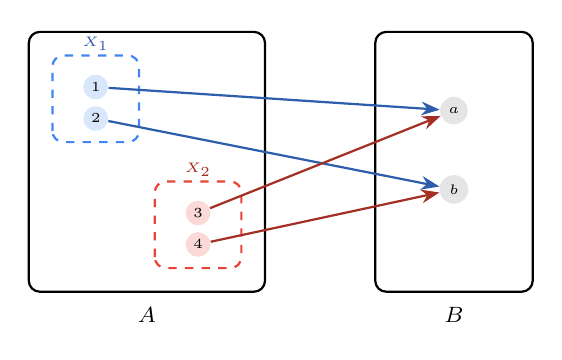
\begin{tikzpicture}[>=Stealth, font=\small]
  \draw[thick, rounded corners] (-0.2, -0.3) rectangle (2.8, 3.0);
  \draw[thick, rounded corners] (4.2, -0.3) rectangle (6.2, 3.0);
  \node[font=\footnotesize\bfseries] at (1.3, -0.6) {$A$};
  \node[font=\footnotesize\bfseries] at (5.2, -0.6) {$B$};

  % X1 box
  \draw[thick, setA, dashed, rounded corners] (0.1, 1.6) rectangle (1.2, 2.7);
  \node[font=\tiny, setA!70!black] at (0.65, 2.85) {$X_1$};
  \node[fill=setA!20, circle, inner sep=1.5pt, font=\tiny] (n1) at (0.65, 2.3) {$1$};
  \node[fill=setA!20, circle, inner sep=1.5pt, font=\tiny] (n2) at (0.65, 1.9) {$2$};

  % X2 box
  \draw[thick, setB, dashed, rounded corners] (1.4, 0.0) rectangle (2.5, 1.1);
  \node[font=\tiny, setB!70!black] at (1.95, 1.25) {$X_2$};
  \node[fill=setB!20, circle, inner sep=1.5pt, font=\tiny] (n3) at (1.95, 0.7) {$3$};
  \node[fill=setB!20, circle, inner sep=1.5pt, font=\tiny] (n4) at (1.95, 0.3) {$4$};

  % B elements
  \node[fill=gray!20, circle, inner sep=2pt, font=\tiny] (a) at (5.2, 2.0) {$a$};
  \node[fill=gray!20, circle, inner sep=2pt, font=\tiny] (b) at (5.2, 1.0) {$b$};

  \draw[->, thick, setA!70!black] (n1) -- (a);
  \draw[->, thick, setA!70!black] (n2) -- (b);
  \draw[->, thick, setB!70!black] (n3) -- (a);
  \draw[->, thick, setB!70!black] (n4) -- (b);
\end{tikzpicture}
\end{center}

Այդ դեպքում՝
\begin{itemize}[nosep]
  \item $X_1 \cap X_2 = \{1,2\} \cap \{3,4\} = \varnothing$։ \checkmark
  \item $f(X_1) = \{f(1), f(2)\} = \{a, b\}$։
  \item $f(X_2) = \{f(3), f(4)\} = \{a, b\}$։
  \item $f(X_1) = f(X_2) = \{a, b\}$։ \checkmark
\end{itemize}

\begin{answerbox}
\textbf{Այո.} Անջատ ոչ դատարկ ենթաբազմությունները կարող են ունենալ հավասար պատկերներ, եթե $f$-ը ինյեկտիվ չէ։
Օրինակ՝ $f(1)=a,\; f(2)=b,\; f(3)=a,\; f(4)=b$, որտեղ $X_1=\{1,2\}$, $X_2=\{3,4\}$։
\end{answerbox}

% ══════════════════════════════════════════════════════════════════
\newpage
\section{Խնդիր 24 — Անջատ բազմությունների նախապատկերներ}
% ══════════════════════════════════════════════════════════════════

\begin{theorybox}[Նախապատկերները պահպանում են բազմությունների գործողությունները]
Ցանկացած $f : A \to B$ ֆունկցիայի և $Y_1, Y_2 \subseteq B$ ենթաբազմությունների համար, \textbf{նախապատկերը}՝
$f^{-1}(Y) = \{x \in A \mid f(x) \in Y\}$, բավարարում է․
\begin{itemize}[nosep]
  \item $f^{-1}(Y_1 \cup Y_2) = f^{-1}(Y_1) \cup f^{-1}(Y_2)$
  \item $f^{-1}(Y_1 \cap Y_2) = f^{-1}(Y_1) \cap f^{-1}(Y_2)$
  \item $f^{-1}(Y_1 \setminus Y_2) = f^{-1}(Y_1) \setminus f^{-1}(Y_2)$
\end{itemize}
Սրանք տեղի ունեն \emph{ցանկացած} ֆունկցիայի համար — ինյեկտիվություն կամ սյուրյեկտիվություն չի պահանջվում։
\end{theorybox}

\begin{problembox}
Ճի՞շտ է արդյոք, որ $f : A \to B$-ի համար, եթե $Y_1 \cap Y_2 = \varnothing$, ապա
$f^{-1}(Y_1) \cap f^{-1}(Y_2) = \varnothing$։
\end{problembox}

\subsection*{Լուծում}

\textbf{Այո}, սա միշտ ճիշտ է։

\begin{proof}
Ենթադրենք $Y_1 \cap Y_2 = \varnothing$։ Մենք օգտագործում ենք $f^{-1}(Y_1 \cap Y_2) = f^{-1}(Y_1) \cap f^{-1}(Y_2)$ նույնությունը։

Քանի որ $Y_1 \cap Y_2 = \varnothing$՝
\[
  f^{-1}(Y_1) \cap f^{-1}(Y_2) = f^{-1}(Y_1 \cap Y_2) = f^{-1}(\varnothing) = \varnothing.
\]

Այլ կերպ կարող ենք ապացուցել ուղղակիորեն։ Ենթադրենք հակառակը, որ գոյություն ունի
$x \in f^{-1}(Y_1) \cap f^{-1}(Y_2)$։ Այդ դեպքում՝
\begin{itemize}[nosep]
  \item $x \in f^{-1}(Y_1) \implies f(x) \in Y_1$։
  \item $x \in f^{-1}(Y_2) \implies f(x) \in Y_2$։
\end{itemize}
Ուստի $f(x) \in Y_1 \cap Y_2 = \varnothing$, ինչը հակասություն է, քանի որ ոչ մի տարր չի պատկանում դատարկ բազմությանը։
\end{proof}

\begin{answerbox}
\textbf{Այո.} Եթե $Y_1 \cap Y_2 = \varnothing$, ապա $f^{-1}(Y_1) \cap f^{-1}(Y_2) = \varnothing$։
Սա բխում է նրանից, որ նախապատկերները պահպանում են հատումները։
\end{answerbox}

\bigskip
\textbf{Հակադրություն պատկերների հետ.}\; Նախապատկերները \emph{միշտ} պահպանում են հատումները՝ $f^{-1}(C \cap D) = f^{-1}(C) \cap f^{-1}(D)$։ Պատկերները՝ \emph{ոչ}, քանի դեռ $f$-ը ինյեկտիվ չէ (տես Խնդիր~19)։ Այս անհամաչափությունը ֆունկցիաների հիմնարար առանձնահատկությունն է։

% ══════════════════════════════════════════════════════════════════
\newpage
\section{Խնդիր 25 — \texorpdfstring{$f(f^{-1}(Y)) \subseteq Y$}{f(f⁻¹(Y)) ⊆ Y}}
% ══════════════════════════════════════════════════════════════════

\begin{theorybox}[Նախապատկերի պատկերը]
$f : A \to B$ ֆունկցիայի և $Y \subseteq B$ ենթաբազմության համար՝
\[
  f(f^{-1}(Y)) \subseteq Y \qquad\text{միշտ տեղի ունի:}
\]
$f(f^{-1}(Y)) = Y$ հավասարությունը տեղի ունի բոլոր $Y \subseteq B$-երի համար այն և միայն այն դեպքում, երբ $f$-ը \textbf{սյուրյեկտիվ} է։

\medskip
\textbf{Ինտուիցիա.}\; $f^{-1}(Y)$-ը ներառում է $A$-ի բոլոր այն տարրերը, որոնք արտապատկերվում են $Y$-ի մեջ։
Կրկին $f$ կիրառելը դրանք հետ է տանում $Y$-ի մեջ, սակայն $Y$-ի որոշ տարրեր կարող են
\emph{նախապատկեր չունենալ}, ուստի դրանք «կորչում են»։

\begin{center}
\begin{tikzpicture}[>=Stealth, font=\small]
  \draw[thick, rounded corners] (-0.2, -0.3) rectangle (2.2, 2.8);
  \draw[thick, rounded corners] (3.5, -0.3) rectangle (6.5, 2.8);
  \node[font=\footnotesize\bfseries] at (1.0, -0.6) {$A$};
  \node[font=\footnotesize\bfseries] at (5.0, -0.6) {$B$};

  % Y subset in B
  \draw[thick, setC, dashed, rounded corners, fill=setC!8] (4.0, 0.2) rectangle (6.0, 2.5);
  \node[font=\scriptsize, setC!80!black] at (5.0, 2.7) {$Y$};

  \node[fill=setB!20, circle, inner sep=2pt, font=\tiny] (y1) at (4.7, 1.8) {$y_1$};
  \node[fill=setB!20, circle, inner sep=2pt, font=\tiny] (y2) at (5.3, 1.2) {$y_2$};
  \node[fill=red!20, circle, inner sep=2pt, font=\tiny] (y3) at (4.7, 0.6) {$y_3$};

  % preimage in A
  \draw[thick, setA, dashed, rounded corners, fill=setA!8] (0.2, 0.8) rectangle (1.8, 2.4);
  \node[font=\scriptsize, setA!70!black] at (1.0, 2.55) {$f^{-1}(Y)$};

  \node[fill=setA!30, circle, inner sep=1.5pt, font=\tiny] (a1) at (0.7, 1.8) {$a_1$};
  \node[fill=setA!30, circle, inner sep=1.5pt, font=\tiny] (a2) at (1.3, 1.4) {$a_2$};

  \draw[->, thick, gray] (a1) -- (y1);
  \draw[->, thick, gray] (a2) -- (y2);

  \node[font=\tiny, red!70!black, align=center] at (4.7, 0.0) {չունի\\նախապատկեր!};
\end{tikzpicture}
\end{center}
Այստեղ $f(f^{-1}(Y)) = \{y_1, y_2\} \subsetneq \{y_1, y_2, y_3\} = Y$։
\end{theorybox}

\begin{problembox}
Ապացուցեք, որ $f : A \to B$ և $Y \subseteq B$-ի համար՝
\[
  f(f^{-1}(Y)) \subseteq Y.
\]
Բերեք օրինակ, որտեղ հավասարությունը տեղի չունի։
\end{problembox}

\subsection*{Լուծում}

\textbf{$f(f^{-1}(Y)) \subseteq Y$-ի ապացույցը։}

Դիցուք $y \in f(f^{-1}(Y))$։ Ըստ պատկերի սահմանման, գոյություն ունի $x \in f^{-1}(Y)$,
այնպիսին, որ $f(x) = y$։ Ըստ նախապատկերի սահմանման, $x \in f^{-1}(Y)$ նշանակում է $f(x) \in Y$։
Հետևաբար $y = f(x) \in Y$։ \qed

\bigskip
\textbf{Օրինակ, որտեղ հավասարությունը խախտվում է։}

Դիցուք $A = \{1\}$, $B = \{a, b\}$, և սահմանենք $f : A \to B$՝ $f(1) = a$։
Վերցնենք $Y = \{a, b\} = B$։

Այդ դեպքում՝
\[
  f^{-1}(Y) = f^{-1}(\{a,b\}) = \{x \in A \mid f(x) \in \{a,b\}\} = \{1\}.
\]
\[
  f(f^{-1}(Y)) = f(\{1\}) = \{f(1)\} = \{a\}.
\]
Բայց $Y = \{a, b\}$։ Ուստի՝
\[
  f(f^{-1}(Y)) = \{a\} \subsetneq \{a, b\} = Y.
\]
$b \in Y$ տարրը չունի նախապատկեր $f$-ի ներքո (քանի որ $f$-ը սյուրյեկտիվ չէ), ուստի այն «կորչում է»։

\begin{answerbox}
\textbf{Ապացույց.} Եթե $y \in f(f^{-1}(Y))$, ապա $y = f(x)$ որևէ $x \in f^{-1}(Y)$-ի համար,
ինչը նշանակում է $f(x) \in Y$, այսինքն՝ $y \in Y$։

\textbf{Հակաօրինակ հավասարության համար.}\; $A = \{1\}$, $B = \{a,b\}$, $f(1) = a$, $Y = B$։
Այդ դեպքում $f(f^{-1}(Y)) = \{a\} \subsetneq \{a,b\} = Y$։

Հավասարությունը տեղի ունի բոլոր $Y$-երի համար այն և միայն այն դեպքում, երբ $f$-ը սյուրյեկտիվ է։
\end{answerbox}

\bigskip
\textbf{Ուղեկցող փաստ.}\; Հակառակ ներդրումը՝ $X \subseteq f^{-1}\bigl(f(X)\bigr)$, միշտ տեղի ունի, իսկ հավասարությունը՝ այն և միայն այն դեպքում, երբ $f$-ը ինյեկտիվ է։ Այս խնդրի $f\bigl(f^{-1}(Y)\bigr) \subseteq Y$ արդյունքի հետ միասին, այս երկու ներդրումները ցույց են տալիս, թե ինչպես են պատկերներն ու նախապատկերները փոխազդում։

\end{document}